\section{Combining learned and exact reduction methods}
\label{sec:hybrid-experts}
The complete-time comparison above retains a fixed setting for the broad request collection. The earlier sparse-seed model has a separate tested use for nonplanar two-loop integrals with higher numerator powers. We therefore combine these methods and measure their complete costs on fresh inputs. Exact formulas handle their supported families first, and independent loop blocks are reduced separately. For the remaining work, the application can use the preceding setting, a fixed sparse boundary, the trained sparse-seed expert, or the original native bounds. Every route retains exact Kira algebra, the supplied master-basis check, and recovery after an unsuccessful attempt.

\subsection{The sparse expert and the complete-time selector}
The sparse expert acts before Kira generates equations. It uses the target numerator powers to select the boundary of a seed region, as defined in Appendix~\ref{app:seed-geometry}. Its validated input domain contains one target in the specified nonplanar massless two-loop box, with seven unit physical powers and numerator rank two, three, or four. We check the ordered denominator and momentum structure before using this expert. Other blocks use the preceding fixed setting within its training ranges and return to original native bounds outside those ranges. The range check also covers numerator ranks above the broad training collection. This domain restriction permits a useful local model without assigning it an unsupported task.

The expert retains its previously trained 32-tree model with maximum depth 2. Its 12 original training requests and 10 model-selection requests precede this experiment. The model predicts log-time ratios for candidate sparse boundaries from 68 inputs: 27 family and target summaries, 40 positive- and negative-power coordinates, and the largest number of negative entries. Tree evaluation uses the saved thresholds and mean leaf values, following the earlier extremely randomized forest construction~\cite{Geurts2006ExtraTrees}. Appendix~\ref{app:hybrid-experts} gives the candidate boundaries and the fresh target batches. The current comparison includes feature calculation, prediction, seed enumeration, input preparation, and every recovery attempt.

We then fit an outer cost model from new complete reduction times. It receives the 51 structural and master-basis inputs of Appendix~\ref{app:total-time}, together with the two auxiliary numerator powers for this ordered family. Its four actions are the four routes listed above. The training cost includes the inner expert's prediction when that route uses it. We use the direct cost split of Eq.~\eqref{eq:total-split}, so the outer model learns which complete route takes less time.

The new collection has 16 training requests and 8 validation requests with separate rational kinematics. Each training action is measured once and each validation action twice. We compare one tree or sixteen trees, maximum depths one through five, and minimum leaf sizes two, four, or seven. Validation first compares the outer prediction with the best constant route. It then compares the resulting application with the best ML-free candidate. Each deployment comparison requires at least 1.5\% less validation cost and no increase in unverified requests. The fixed sparse candidate retains the boundary selected in the earlier expert study. Current validation compares that candidate with the preceding setting and original native bounds to select the ML-free control. The selected control is a fixed sparse-seed boundary. Validation enables the outer 1-tree model, with maximum depth 2 and minimum leaf size 4. The selected validation cost is 52.826 seconds, compared with 55.917 seconds for the ML-free control. These model-selection results precede the reserved test.

\subsection{Fresh complete-workflow comparison}
The reserved comparison contains twenty-four nonplanar target requests and ten compatibility requests. The nonplanar requests cover every distribution of numerator ranks two through four across the two auxiliary coordinates at two new kinematic profiles. Eight of these requests use index vectors absent from the new outer-model training and validation collection. The earlier inner expert has a separate training history, which includes some of these added shapes. The ten compatibility requests include native coupled families through three loops, independent products through thirteen loops, and a thirteen-loop analytic case. We freeze the expert weights, outer model, domain checks, and decisions before testing. Each request uses three repetitions with rotated method order on one worker. The preceding application runs through its actual entry point. The fixed control disables both learned predictions, while all routes retain exact coefficient checks and the same native resource limits.

The integrated application verifies 34 of 34 requests in all three repetitions, and invokes learned prediction on 24. For 34 matched requests, the integrated method takes 156.290 seconds and the preceding complete-time application takes 161.592 seconds. This gives 3.3\% less time, with ratio 0.967 and repetition interval $[0.950,1.003]$. For 24 matched requests, the integrated method takes 136.956 seconds and native seed bounds takes 225.338 seconds. This gives 39.2\% less time, with ratio 0.608 and repetition interval $[0.584,0.640]$. For 24 matched requests, the integrated method takes 136.956 seconds and the validation-selected ML-free control takes 143.079 seconds. This gives 4.3\% less time, with ratio 0.957 and repetition interval $[0.925,0.998]$. The comparison with the selected ML-free control resolves an added saving from learned decisions beyond the measured repetition variation. For 8 matched requests, the integrated method takes 52.876 seconds and the validation-selected ML-free control takes 51.685 seconds. This gives 2.3\% more time, with ratio 1.023 and repetition interval $[0.974,1.109]$. For 8 matched requests, the integrated method takes 52.876 seconds and the preceding complete-time application takes 48.131 seconds. This gives 9.9\% more time, with ratio 1.099 and repetition interval $[1.066,1.194]$. These added index patterns expose a remaining transfer limit for the outer selector.

\begin{table}[!htbp]\centering\small
\caption{Complete hybrid comparison. The first-pass time includes one attempt at every requested calculation. Ratios use sums of request medians on matched exact completions. The fixed setting is selected from the three declared ML-free candidates on validation data.}
\label{tab:hybrid-experts}
\begin{tabular}{@{}lrrrr@{}}\toprule
Method & Verified & First pass (s) & Integrated/method & Failed calls\\\midrule
Preceding application & 34/34 & 162.721 & 0.967 & 0\\
Native bounds & 34/34 & 243.584 & 0.636 & 0\\
Selected ML-free control & 34/34 & 165.651 & 0.961 & 48\\
Integrated method & 34/34 & 159.543 & 1.000 & 0\\
\bottomrule\end{tabular}\end{table}
\begin{figure}[!htbp]\centering
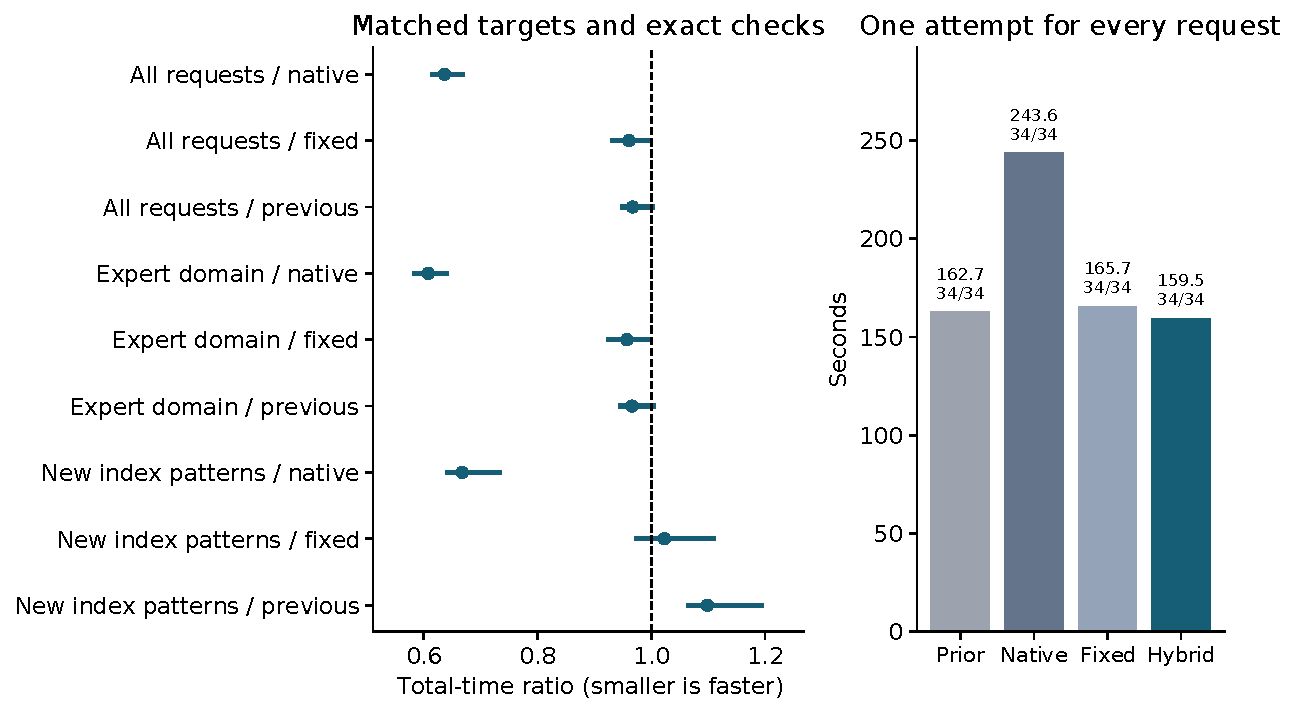
\includegraphics[width=\linewidth]{paper_figures/hybrid_expert_selection.pdf}
\caption{The left panel gives complete-time ratios for all matched requests, the sparse-expert domain, and the additional index patterns absent from outer-model training. The fixed control isolates the added learned decision. The line at one marks equal time, and horizontal bars show paired repetition variation. The right panel includes one attempt for every request and labels verified coverage. Prior and Hybrid denote the preceding and integrated applications.}
\label{fig:hybrid-experts}
\end{figure}
Across all recorded attempts and repetitions, the integrated method takes 476.353 seconds, compared with 493.287 seconds for the ML-free setting and 487.815 seconds for the preceding application. The 128 new training and validation measurements take 1033.449 timed seconds; outer-model fitting takes 12.241 seconds. Independent reference preparation for the reserved requests takes 908.971 seconds outside the application timers. The earlier expert training and checked master-basis preparation are additional prior costs.

The comparison measures use with an existing checked basis and includes model loading, prediction, equation generation, algebra, exact checks, and recovery. The direct learned result applies to the specified nonplanar family and numerator range. The compatibility checks verify the retained routes on their stated families; the broader baseline comparison above remains a separate experiment. The application keeps native row and equation choices. These finite tests establish no globally fastest reduction or coverage of arbitrary high-loop scattering.
